% This is text associated with the open textbook "Open Electromagnetics"
% See immediately below for author, date
% This work is licensed under the Creative Commons Attribution-ShareAlike 4.0 International License. (CC BY-SA 4.0) 
% To view a copy of the license, visit http://creativecommons.org/licenses/by-sa/4.0/

%ORB TITLE TE Reflection in Non-magnetic Media
%ORB AUTHOR 0        # S.W. Ellingson, Virginia Tech (ellingson@vt.edu)
%ORB DATE 20191119   # yyyymmdd
%ORB ABSTRACT 

\label{m0171_TE_Reflection_Nonmagnetic_Media} % <-- Must match name of this file and module directory name.  Don't mess with this!
\index{transverse electric|(}

Figure~\ref{m0171_fObliqueTE} shows a TE uniform plane wave incident on the planar boundary between two semi-infinite material regions.
%
\begin{figure}[b!]
\begin{center}
\pdftooltip{{  % note double braces
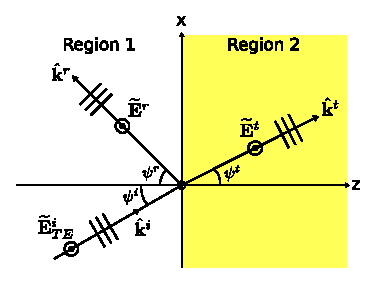
\includegraphics[width=0.8\columnwidth]{modules/m0171_fObliqueTE.eps} 
% https://commons.wikimedia.org/wiki/File:TE-polarized_upw_incident_on_planar_boundary.svg
}}{For a z-x Cartesian coordinate system, a TE plane wave approaches planar boundary at an oblique angle. The reflected wave in region 1 and the transmitted wave in region 2. Electric field is out of page.}
\end{center}
\centerline{\scriptsize 
\copyright~\hyperref[m0171_fObliqueTE_Credit]{C.\ Wang} 
\href{https://creativecommons.org/licenses/by-sa/4.0/}{CC BY-SA 4.0} 
} 
\caption{
\label{m0171_fObliqueTE}
A TE uniform plane wave obliquely incident on the planar boundary between two semi-infinite regions of lossless non-magnetic material.
}
\end{figure}
%  
In this case, the reflection coefficient is given by:
%
\begin{equation}
\Gamma_{TE} = \frac{\eta_2\cos\psi^i-\eta_1\cos\psi^t}{\eta_2\cos\psi^i+\eta_1\cos\psi^t}
\label{m0171_eGTE}
\end{equation}
%
where $\psi^i$ and $\psi^t$ are the angles of incidence and transmission (refraction), respectively; and $\eta_1$ and $\eta_2$ are the wave impedances in Regions~1 and 2, respectively.
Many materials of practical interest are non-magnetic; that is, they have permeability that is not significantly different from the permeability of free space.  In this section, we consider the behavior of the reflection coefficient for this class of materials.

To begin, recall the general form of Snell's law: 
\index{Snell's law}
%
\begin{equation}
\sin{\psi^t} = \frac{\beta_1}{\beta_2}\sin\psi^i
\label{m0171_eSLNM}
\end{equation}
%
In non-magnetic media, the permeabilities $\mu_1$ and $\mu_2$ are assumed equal to $\mu_0$.  Thus:
%
\begin{equation}
\frac{\beta_1}{\beta_2} = \frac{\omega\sqrt{\mu_1\epsilon_1}}{\omega\sqrt{\mu_2\epsilon_2}} = \sqrt{\frac{\epsilon_1}{\epsilon_2}}
\end{equation}
%
Since permittivity $\epsilon$ can be expressed as $\epsilon_0$ times the relative permittivity $\epsilon_r$, we may reduce further to:
%
\begin{equation}
\frac{\beta_1}{\beta_2} = \sqrt{\frac{\epsilon_{r1}}{\epsilon_{r2}}}
\end{equation}
%
Now Equation~\ref{m0171_eSLNM} reduces to:
%
\begin{equation}
\sin{\psi^t} = \sqrt{\frac{\epsilon_{r1}}{\epsilon_{r2}}} \sin\psi^i
\end{equation}
%
Next, note that for any value $\psi$, one may write cosine in terms of sine as follows:
%
\begin{equation}
\cos{\psi} = \sqrt{1-\sin^2{\psi}}
\end{equation}
%
Therefore, 
%
\begin{equation}
\cos{\psi^t} = \sqrt{1-\frac{\epsilon_{r1}}{\epsilon_{r2}} \sin^2\psi^i }
\label{m0171_eCpt}
\end{equation}
%
Also we note that in non-magnetic media
%
\begin{flalign}
\eta_1 &= \sqrt{\frac{\mu_1}{\epsilon_1}} = \sqrt{\frac{\mu_0}{\epsilon_{r1}\epsilon_0}} = \frac{\eta_0}{\sqrt{\epsilon_{r1}}} \\
\eta_2 &= \sqrt{\frac{\mu_2}{\epsilon_2}} = \sqrt{\frac{\mu_0}{\epsilon_{r2}\epsilon_0}} = \frac{\eta_0}{\sqrt{\epsilon_{r2}}} 
\end{flalign}
%
where $\eta_0$ is the wave impedance in free space.
Making substitutions into Equation~\ref{m0171_eGTE}, we obtain:
%
\begin{equation}
\Gamma_{TE} = \frac{\left(\eta_0/\sqrt{\epsilon_{r2}}\right)\cos\psi^i-\left(\eta_0/\sqrt{\epsilon_{r1}}\right)\cos\psi^t}{\left(\eta_0/\sqrt{\epsilon_{r2}}\right)\cos\psi^i+\left(\eta_0/\sqrt{\epsilon_{r1}}\right)\cos\psi^t}
\end{equation}
%
Multiplying numerator and denominator by $\sqrt{\epsilon_{r2}}/\eta_0$, we obtain:
%
\begin{equation}
\Gamma_{TE} = \frac{\cos\psi^i-\sqrt{\epsilon_{r2}/\epsilon_{r1}}\cos\psi^t}{\cos\psi^i+\sqrt{\epsilon_{r2}/\epsilon_{r1}}\cos\psi^t}
\end{equation}
%
Finally, by substituting Equation~\ref{m0171_eCpt}, we obtain:
%
\begin{equation}
\boxed{
\Gamma_{TE} = \frac{\cos\psi^i-\sqrt{\epsilon_{r2}/\epsilon_{r1}-\sin^2\psi^i}}
                   {\cos\psi^i+\sqrt{\epsilon_{r2}/\epsilon_{r1}-\sin^2\psi^i}}
}
\label{m0171_eGTEi}
\end{equation}
%
This expression has the advantage that it is now entirely in terms of $\psi^i$, with no need to first calculate $\psi^t$.

Using Equation~\ref{m0171_eGTEi}, we can see how different combinations of material affect the reflection coefficient.
First, we note that when $\epsilon_{r1}=\epsilon_{r2}$ (i.e., same media on both sides of the boundary), $\Gamma_{TE}=0$ as expected.
When $\epsilon_{r1}>\epsilon_{r2}$ (e.g., wave traveling in glass toward air), we see that it is possible for $\epsilon_{r2}/\epsilon_{r1}-\sin^2\psi^i$ to be negative, which makes $\Gamma_{TE}$ complex-valued.  This results in \emph{total internal reflection}, 
\index{total internal reflection}
and is addressed elsewhere in another section.
When $\epsilon_{r1}<\epsilon_{r2}$  (e.g., wave traveling in air toward glass), we see that $\epsilon_{r2}/\epsilon_{r1}-\sin^2\psi^i$ is always positive, so $\Gamma_{TE}$ is always real-valued.

Let us continue with the $\epsilon_{r1}<\epsilon_{r2}$ condition.
Figure~\ref{m0171_fTEnmG} shows $\Gamma_{TE}$ plotted for various combinations of media over all possible angles of incidence from 0 (normal incidence) to $\pi/2$ (grazing incidence).
%
\begin{figure} % <--- "[b]" for first figure in section *only*; delete for 2nd and subsequent figures
\begin{center}
\pdftooltip{{  % note double braces
\includegraphics[width=2in,angle=-90,origin=c]{modules/m0171_fTEnmG.eps} 
% https://commons.wikimedia.org/wiki/File:M0003_fBarMagnet.svg
}}{A plot of reflection coefficient versus angle of incidence in degrees. Angle plotted from 0 to 90 degrees and coefficient from -1 to 1. Three curves from the highest coefficient to lowest have ratios 2, 10, and 100. The curves become progressively flatter and closer to -1 as the ratio increases.}
\end{center}
%\centerline{\scriptsize 
%\copyright~\hyperref[m0003_fBarMagnet_Credit]{Y.\ Qin} 
%\href{https://creativecommons.org/licenses/by/3.0/}{CC BY 3.0} 
%} % \centerline 
\caption{
\label{m0171_fTEnmG}
The reflection coefficient $\Gamma_{TE}$ as a function of angle of incidence $\psi^i$ for various media combinations.  Curves are labeled with the ratio $\epsilon_{r2}/\epsilon_{r1}$.
}
\end{figure}
%
We observe:
%%%%%%%%%%%%%%%%%%%%%%%%%%%%%%%%%%%%%%%%%%%%%%%
%ORB HIGHLIGHT
\begin{mdframed}[backgroundcolor=yellow!20,nobreak=true] 
In non-magnetic media with $\epsilon_{r1}<\epsilon_{r2}$, $\Gamma_{TE}$ is real-valued, negative, and decreases to $-1$ as $\psi^i$ approaches grazing incidence.
\end{mdframed}
%%%%%%%%%%%%%%%%%%%%%%%%%%%%%%%%%%%%%%%%%%%%%%%

Also note that at any particular angle of incidence, $\Gamma_{TE}$ trends toward $-1$ as $\epsilon_{r2}/\epsilon_{r1}$ increases.
Thus, we observe that as $\epsilon_{r2}/\epsilon_{r1}\to\infty$, the result is increasingly similar to the result we would obtain for a perfect conductor in Region~2.

\index{transverse electric|)}

